\documentclass[a4paper]{article}
\usepackage{iemss}
\usepackage[pdftex]{graphicx}
\usepackage[authoryear]{natbib}
\usepackage[labelfont=bf,textfont=sf,labelsep=period]{caption}
\usepackage[english]{babel}

% extra packages not in the template
% Don't color hyperlinks
\usepackage{wrapfig}
\usepackage{paralist}
\usepackage[draft]{hyperref}
\usepackage{amsmath}
\usepackage[printonlyused,withpage]{acronym}
\usepackage{sansmath}

% \RequirePackage{lineno} % for line numbers

\pdfpagewidth=210 true mm
\pdfpageheight=297 true mm

\renewcommand{\rmdefault}{phv} % Arial
\renewcommand{\sfdefault}{phv} % Arial

\bibpunct{[}{]}{;}{a}{,}{,~}

\pagestyle{IEMSSheadings}



\DeclareRobustCommand{\orderof}{\ensuremath{\mathcal{O}}}
\DeclareRobustCommand{\threedi}{3Di }

% Text to appear in the header of the pages
\IEMSShead{Baart et al. / Interactive web-based flood modeling}

\graphicspath{{figures/}}
\DeclareGraphicsExtensions{.pdf,.png,.jpg}

\title{Interactive web based flood modeling at country wide scale and planter size resolution.}


% Authors Names and Affiliations:  Two spaces below the title, 10 pt
% Arial, Upper and Lower Case, underline author presenting
% paper and  provide his/her email address


\author{\underline{F. Baart}
  \address[A1]{\it{Deltares,
      Rotterdamseweg
      Delft, The Netherlands (fedor.baart@deltares.nl, arthur.vandam@deltares.nl, gennadii.donchyts@deltares.nl)}},
  K. K. Ha
  \address[B1]{\it{Nelen \& Schuurmans,
      Zakkendragerssteeg,
      Utrecht, The Netherlands (jack.ha@nelen-schuurmans.nl, martijn.siemerink@nelen-schuurmans.nl)}},
  A. van Dam \addressmark[A1],
  G. Donchyts \addressmark[A1],
  M. Siemerink \addressmark[B1]
}


\begin{document}
% make sure everything is sans-serif, including math
\sffamily
\sansmath


\begin{abstract}
  The flooding of rural and urban areas is an increasing hazard to society. Accurate and timely predictions are essential for the water manager to prepare and respond to these hazards.
  Predicting flooding requires a numerical model that represents the physical processes (rain, evaporation, infiltration, overland flow, groundwater flow). This model, fed with measurements, and possible measures, calculates the expected flooding.
  The traditional modelling process consists of a three step process: schematization setup, model running and post-processing, with a total feedback time of hours.  This process is suitable for confirmatory modelling. Most of the time, models are applied exploratory, requiring a different workflow.
  Enabling exploratory modelling requires a shift in utilisation of the modelling instrument. Stakeholders are in control and together evaluate ideas by interacting with the model through a mobile compatible website, supported by the modellers’ expertise. Enabling this type of interactive modelling requires a new level of performance.
  The \threedi platform, in which the new approach was applied, consists of a new flooding and hydrological model (1D/2D) with a corresponding cloud based infrastructure. Applications in rural and urban areas of \orderof(1000km2) at a resolution of \orderof(0.1m) have shown its capabilities for both exploratory and confirmatory modelling.
  The ambition that every component should be at least a 100 times faster than the previous approach, resulted in several advancements, both in the numerical engine and the software that interacts with the user and pushes the data to the web. Here we show advancements in the architecture and model communication.

\end{abstract}
\begin{keyword}
\end{keyword}

\maketitle


\section{Introduction}
The flooding of rural and urban areas is an increasing hazard to society. Accurate and timely predictions are essential for the water manager to be able to carefully plan, design and control the effects of flooding hazard.
For the prediction of these flooding hazards requires a numerical model that represents the physical processes (rain, evaporation, flow, infiltration). This model is fed with measurements from current or historic events. The results of these calculations, the expected flooding, is used for damage estimates, dike design, spatial and emergency planning and for coordinating response efforts. Several challenges required an innovative redesign of both the numerical model and the information infrastructure where it is nested within.

These challenges arise from the movement towards more modern working methods and the ever increasing data volumes. The working methods are changing on different aspects.
\begin{itemize}
\item \emph{Mono-disciplinary versus integrated} Models used to be created by one or few people working in the same discipline. The challenge now is to model the integrated environment, which can best be approached as a community \citep{Voinov2010} of different disciplines.
\item \emph{Confirmatory versus exploratory} From assuming that the model is valid and can be used for hypothesis testing to realizing it's a made-up simplification of reality \citep{Oreskes1994} that can be used to explore possibilities.
\item \emph{Passive versus interactive} Moving from the pre-processing, wait a few hours, post-processing cycle towards a millisecond feedback loop with high resolution and connected physical processes. The challenge here is to move from the scale of a square kilometer \citep[for example][]{Losasso2008} to the scale of small country.
\item \emph{Solitary versus social} The solitary modeler creating static pictures for a 600 page report describing all the different scenarios to a group of stakeholders in control \footnote{preferably with guidance from domain experts} of a model running simultaneous on their mobile devices and a big screen in the control room.
\end{itemize}

The amount of data involved in preparing the model is rapidly increasing. There is an increase in supply of data caused by the ever growing measurement resolution and spatial coverage. For example the topology of waterbodies at a spatial coverage of a small country are used to determine if the water will find its way into ones neighborhood. The topography and infiltration rate at a spatial resolution of a planter determine if the water will flow to ones backyard or the neighbors.
This resulted in the question how can we design a platform that is suitable for this new modeling approach and meets the corresponding challenges.

% Several attempts have been made to enable the movement towards these new working methods and increased data volumes.
% Refs Numerical (adaptive mesh): overview
% Interactive models: IRF: ESMF, OpenMI
% Social modelling:
% Web based modelling:

The \threedi  platform, in which these approaches and several new ones are applied, consists of a new overland flooding model (1D/2D) and a corresponding infrastructure that has been applied for interactive web-based modeling of rural and urban areas at coverages of \orderof(1000km2) at a resolution of \orderof(0.1m). Here we describe the advances in the numerical methods, architecture and visualization techniques that were used to create the platform.

% The advances on a numerical level, by implementing a quad tree structure allowing only the relevant physics to be computed, resulting in an order of magnitude speedup have been previously presented. Here we present the new architecture and it's underlying components, resulting in the advances in model interaction and scalability.
% The new multi-tier infrastructure was designed under the following conditions:
% Every aspect of the system should be 100 times faster than the previous approach.
% The main end user is the water-manager, who is assumed to only know how to use a browser and likes to present realistic looking results.
% The modeling should be interactive and social, meaning that multiple people can interact with the same running model at the same time.
% The system should be able to run both in private and public clouds. The numerical model should be able to run on a single computer on a supercomputer and in the cloud.
% The main interface is a mobile compatible website. The model results are rendered on the client in a html5 web map using both bitmap and vector graphics. The user can interact with the model in several ways, for example by changing properties of hydraulic structures, water levels, discharge locations, rain events. The browser transforms these interactions into messages which are pushed back to the model through websockets. Model results are also pushed to the browser using websockets and on request through a Web Map Service (WMS) extended with time support.
% The web application server forwards the websockets messages back and forth between the browser and the model. This application also keeps track of authorization, authentication, user preferences and the social aspects, who is watching which model, who is in control.
% The numerical model was adapted to an interactive model by implementing the low level, non invasive BMI interface. This interface makes the numerical model adhere to the Hollywood principle (don't call us, we'll call you): the control of the initialize, update and finalize steps are called from outside of the numerical model. All variables of the model can be accessed through direct or shared memory access, allowing for communication within nanoseconds. The numerical model can be run as a command line executable (for operational runs), in a GUI (for schematization design), as a shared library (for data exchange) and as a message publisher/puller (for interaction). A separate tool generates photo-realistic renderings in 3D stereo for presentation purposes. The messaging publisher module, which works for any BMI compliant model, allows to push results to the browser at a rate of over 20 time per second and a latency of under 50ms.
% A provisioning module is used to quickly deploy new updates of models schematization and to scale when more running models or WMS servers are required. Models can run at cloud providers and at the central server. Model schematizations are kept under distributed version control so that updates can be pushed and different versions of the same model can be used.
% The new platform has been deployed at several locations in the Netherlands and in Singapore. In preliminary tests we found that the model has skill comparable to previous models. Setting the bar for performance a few order of magnitudes higher resulted in new ideas instead of improved existing ideas. A major part of the platform (model messaging, WMS server) has been released open source because it can also be used with other models. The numerical model is shared within a small community.
% By solving the challenges new challenges arise. The new challenges are technical and social. How can we dynamically filter out the most relevant information from the platform as the bandwidth and browsers rendering power of the mobile browsers is limited and varying. The shift towards social and exploratory modeling and away from the modeler "in control" require new best practices. How do we make sure information is used correctly? How "true" is the information perceived?

\section{Numerical model}
The computational core originates from core components of the {SOBEK} 1D2D flooding software \citep{Stelling2006}, and has undergone three major transformations. \begin{inparaenum}
\item a streamlining of the software architecture to offer access to the memory of a running model,
\item overland flow at subgrid scale and
\item inclusion of hydrological processes in the subsoil also at subgrid scale.
\end{inparaenum}

The traditional standalone flooding program and its integrated \ac{GUI} have been split into dedicated components. Most importantly, the core library with all numerical algorithms and I/O. On top of this core library are independent ways of addressing the core: a light-weight interface library that exposes the \ac{API}, and the original technical \ac{GUI} that acts as a sandbox for early developments.
The core and \ac{API} offer powerful new functionality for direct and fast interaction using introspection (described in \autoref{sec:coupling} and the Hollywood-principle.

By introspection, the outside world (e.g., a Python-based website, a C\#-\ac{GUI}, a MATLAB-script) can examine model state at run time. More specifically: get current water levels and flow fields, current running state of water pumps and other structures, active meteorological forcings. Each of these state variables can just as easily be \emph{set} as they are \emph{read}. The \ac{API} exposes memory pointers to relevant model state variables. The model will directly 'feel' and use its new state.

The freedom of changing model state is possible due to the core and \ac{API} adhering to the Hollywood Principle: ``Don't call us, we'll call you''. The core or model does not run itself, but instead is instructed by the outside world. Typically, the timeloop from a conventional program is extracted and moved to the calling application; only the single timestep remains in the core.

In several workshops, model coupling frameworks \citep[see][for an overview]{Jagers2010}, have agreed on the minimal interface that makes a model adhere to the Hollywood principles, by exposing the following methods:

\begin{enumerate}
\item \textbf{initialize()}: Load and initialize a model from file.
\item \textbf{run($\Delta t$)}: Run a single timestep.
\item \textbf{finalize()}: Finalize the model, memory cleanup, file flushing, statistics reporting.
\end{enumerate}

\begin{wrapfigure}[19]{r}{0.5\textwidth}
\centering
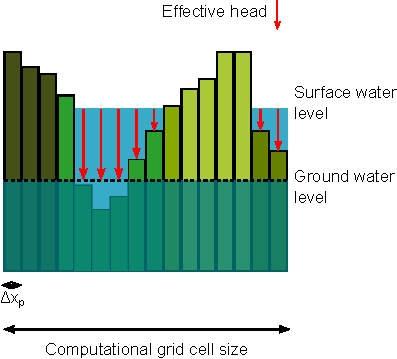
\includegraphics[width=0.48\textwidth]{subgrid_hydrology}
\caption{Subgrid infiltration into heterogeneous landscape.}
\label{fig:figure2}
\end{wrapfigure}

In between these interface calls, the model state may be changed from outside and the core should support that. The library is loaded and can remain a running process for a long time, for many different models.. A positive side-effect of implementing this interface is that it may reveal subtle inconsistencies in existing code, for example when initializing different models after one another: incomplete cleanup of previous settings, already allocated memory, unclosed file pointer.


The power and elegance of the subgrid concept is now also proving itself for the hydrological processes in the subsoil. The planter size pixel resolution of the digital terrain maps for detailed evaluation of overland flow friction and water storage is described in \citet{Stelling2012}. Coupling the 2D grid with 1D channels and controllable structures enables greater detail in civilized regions.


Another important influence on potential flooding is the storage of water in the subsoil, or the lack thereof. The change in surface water volume is driven by several familiar processes:
\[
\Delta V_\mathrm{surface\ water}=(Q_\mathrm{overland} + Q_\mathrm{precipitation} - Q_\mathrm{infiltration} - Q_\mathrm{evapo(transpi)ration} + Q_\mathrm{drainage})\cdot\Delta t
\]
Infiltration, evaporation and drainage are now also evaluated at pixel resolution, whereas the computational grid cells are larger and ensure high performance.

The heterogeneous landscape and land use (be it it urban and/or rural) are specified in the model as gigapixel bitmaps for soil types, crop types, drainage resistance and maximum infiltration. Consider the basic head-dependent linear infiltration in (\ref{eq:qinf}) as an example.
%
\begin{equation}
\label{eq:qinf}
Q_\mathrm{infiltration}= \sum_{\mathrm{pixels}\ i,j} \frac{\min(0, \zeta_\mathrm{sw}-\max(h_\mathrm{gw}, d_{i,j}))}{\mathrm{resistance}_{i,j}}\Delta x_p \Delta y_p,
\end{equation}
where $\zeta_\mathrm{sw}$ and $h_\mathrm{gw}$ are surface and ground water level, respectively, and $d_{i,j}$ is the surface/bed level of pixel $(i,j)$. Notice how dry pixels (higher land) do not amount to the total infiltration.


Note that this specific type of head-dependent infiltration rate in can be chosen freely, but the fact that it uses pixel-resolution soil characteristics is what is important here.

%
These advances in the numerical model allow the model to act as a component in the interactive web-based model environment that will be described in the next section.

\section{Architecture}
\begin{wrapfigure}[12]{l}{0.5\textwidth}
  \centering
  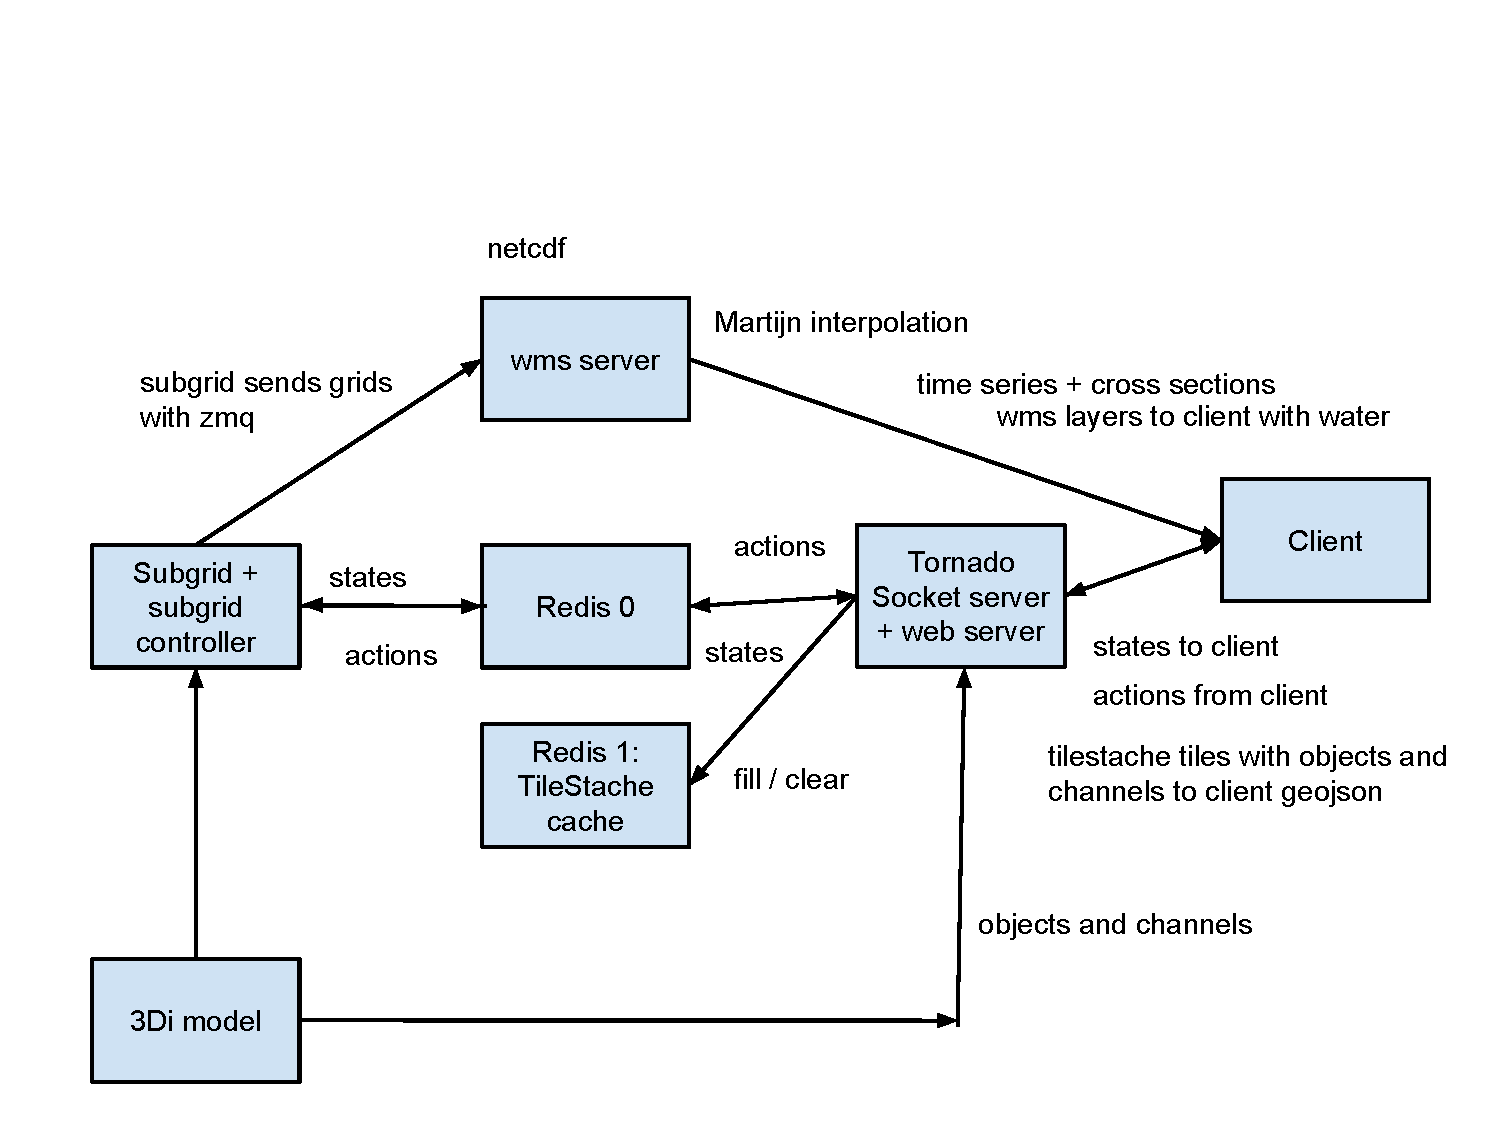
\includegraphics[width=0.48\textwidth]{architecture}
  \caption{Architecture overview}
  \label{fig:arch}
\end{wrapfigure}

To enable social and interactive modeling through a map environment the most logical choice was to use a web based environment. Over the last years this choice has become easier through the large list of advancements for browser based applications.  An overview of the architecture is given in \autoref{fig:arch}. Notice how the architectural follows the general Model View Controller pattern \citep{GOF2004}. On a high level the architecture follows is classic. In this section we will describe the lower level, yet important,  technical innovations that made the application of this architecture successful.

\begin{wrapfigure}[16]{r}{0.5\textwidth}
  \centering
  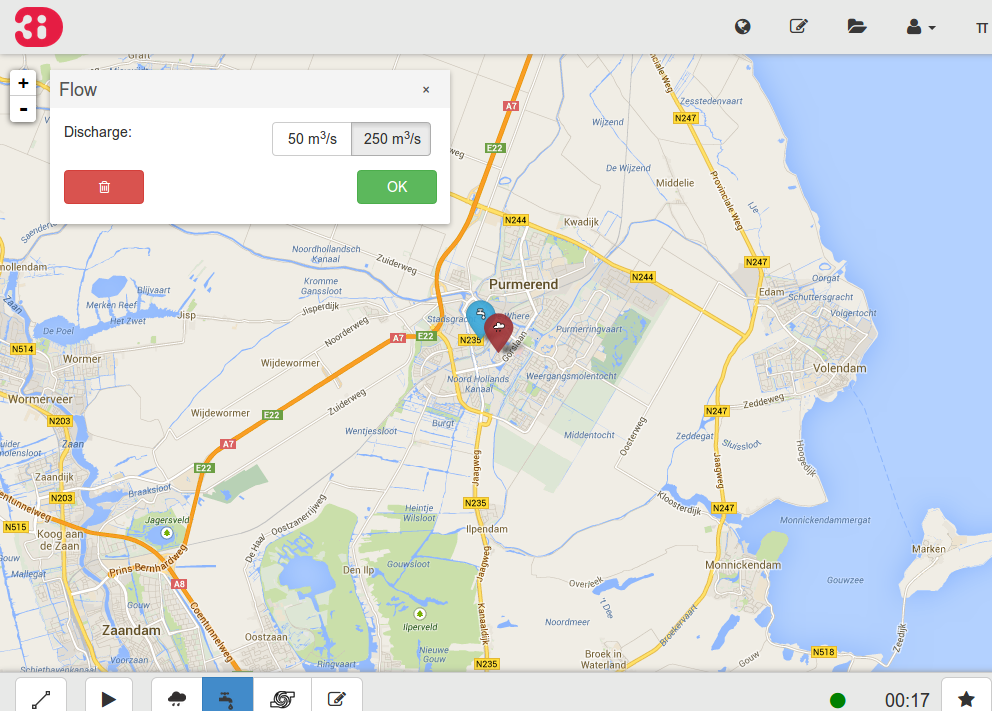
\includegraphics[width=0.48\textwidth]{webgui}
  \caption{Web \ac{GUI}}
  \label{fig:gui}
\end{wrapfigure}

The end-users, interact with the web based \ac{GUI}. The design philosophy is minimalistic, allowing little room for user mistakes. For example manholes can only be placed inside the model domain, and can be controlled by only two different discharge settings (normal and extreme discharge). Sessions with groups of end-users resulted in the idea that this interface was the most usable. The design goals of providing freedom to explore together with high resolution high frequency model output, yet without the insinuation that the model results are ``true'' proves to be challenging. Many end-users confuse high resolution, detailed tuning parameters and higher frequency results with higher accuracy.

Several challenges arise when preparing a model for a web-based use. One of the differences when comparing a desktop user to a web-based user is the short attention span. If no indication of progress is given for longer than two second users will start reloading, clicking erratically or will just close the website as a whole searching for a new ``frisson'' \citep{Carr2011}.

To make sure that the model is ready to run when a user arrives and no time is lost with starting up, initializing, reading files a lot of attention is given to the provisioning of the model. Provisioning in this context is preparing a model controller so that it starts it's computation on request. Machines are prepared and put on hold at one of the \ac{IaaS} providers (such as Amazon). These machines are prepared with a container that contains the model schematization, tables and grids and hot restart files. The tables, grids and restart files are read into memory so that the model is ready to start its computation when it is needed. This results in a time between a user logging in and a model start below 5 seconds.

Interaction is another challenge where timing is crucial. When a user interacts with the model, for example places a discharge point, turns on a pump or lowers an orifice she expects a response within a second. This short feedback loop is achieved using several techniques. Using the regular \ac{HTTP} GET Request is too slow in this case. To reduce communication we use a chain of direct connections. This starts with a websocket \citep{w3c2010} connection between the message broker and the browser. The model controller gets notified directly of user interactions. These interactions are collected in a separate thread and pushed into the model on every timestep. These timesteps have to be kept shorter than in a classical model run. A timestep resulting in a computation time of \si{100}{\mili\second} is common. After a model timestep the chain is inverted. The model pushes it's arrays back in the direction of the browser, which is subscribed to these events and can directly visualize the results. This message broker approach allows interactions with a feedback time in the order of \si{100}{\mili\second}, which gives a good sense of interactivity.

As a final challenge there is the social aspect of modeling. Several group sessions with different settings have been tried. The current setup is that the model is run in a channel, like in a chat room. Multiple people can join the model run. One person is in control and others can view and zoom in on the same model run. Other users can request control of the model. The sessions worked best when a topic expert, not necessary a modeler was present in the session.

\subsection{Data sources }
\begin{itemize}
  \item lidar
  \item rain example
  \item structures/levees
\end{itemize}

\section{Coupling}
\label{sec:coupling}

\begin{itemize}
  \item raster
  \item quad unstructured
  \item 1d network
  \item structure tables
\end{itemize}

\subsection{BMI}

Basic Model Interface Wrapper
The \ac{BMI} is a low level API designed access both control and data access functions of the model engine component. It is similar to the type introspection used in many programming languages, however, instead of the class types \ac{BMI} provides access to the model variables, including their attributes such as data type, unit of measure, input or output role. To provide full access to the internals of the internal model state the following function types should be implemented: model control, model information, variable information, variable getter and setter and grid information. The \ac{BMI} API is quite compact and does not require much effort to implement it in the model. However, it can be quite time consuming to continuously extend access to the model variables in programming languages such as fortran. To simplify this maintenance process we have implemented an automated way to add or remove model variables via \ac{BMI}. The automation was added using Python script and Mako template engine (Figure 1).


\begin{figure}[h]
  \centering
  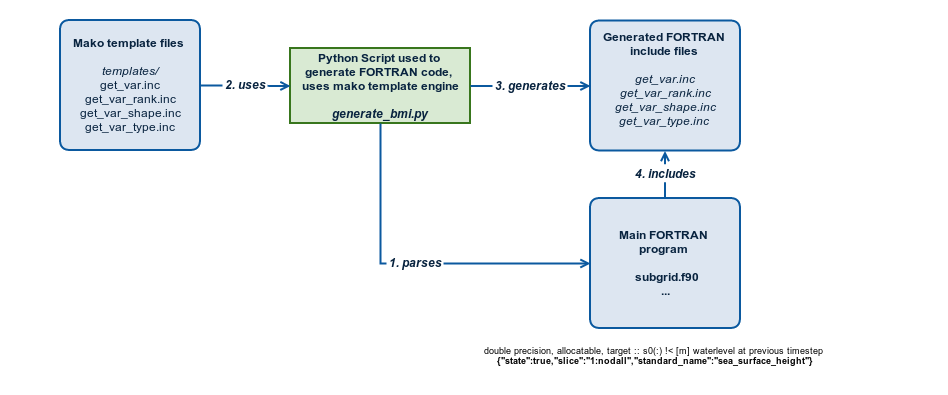
\includegraphics[width=10cm]{bmi_3di}
  \caption{Basic Model Interface template}
  \label{fig:bmi}
\end{figure}

Figure 1: Automatic generation of the include files for \ac{BMI} support

The Mako template files used to generate FORTRAN include all code necessary to expose all required external functions of the model engine shared library. This library is then used by the 3Di model wrapper (developed using Python and ctypes) to control model.

The approach described above significantly decreased costs of change required to maintain \ac{BMI} support in the 3Di model.

Additionally to the standard functions we had to extend BMI with support for simple compound data types (C structures using only simple fields). This was necessary to simplify access to the higher level model entities such as hydraulic structures (e.g. pumps, weirs, culverts).

\subsection{MMI}
\begin{itemize}
  \item message interface
  \item serialization
  \item comparison to other interfaces
\end{itemize}
\subsection{Websockets}
\begin{itemize}
  \item Advantages of push for models
  \item Serialization
\end{itemize}
\section{Visualization}
\subsection{Ravensburger }
\begin{itemize}
  \item performance comparison
  \item WMS/TWMS coupling
\end{itemize}
\subsection{Interpolation}
Interpolation Martijn

The 3Di platform enables a more exploratory approach to modeling, serving a wide variety of end-users. The variety of end-users exposes the numerical model to non-technical users with little understanding of implemented numerical schemes. Some artefacts resulting from the numerical schemes are therefore filtered and smoothed using an interpolation method. Artefacts include squared water depth visualization and water present on two sides of a levee within one calculation cell. The filtering and smoothing reduces the need for prior knowledge of numerical modeling.

The numerical core of the 3Di platform is based on a subgrid calculation method (Stelling, 2012). The hydrodynamic calculations are performed on a non-uniform grid (quadtree ordering), with use of high resolution \ac{DEM} information as input. Flow variables, such as water levels and flow velocities, are available on the calculation grid, which reduces storage costs. The resulting adaptive storage of flow variables results in artefacts after plotting them on the high resolution \ac{DEM} rasters. Figure 1a shows the occurring artefacts.


\begin{figure}[h]
  \centering
  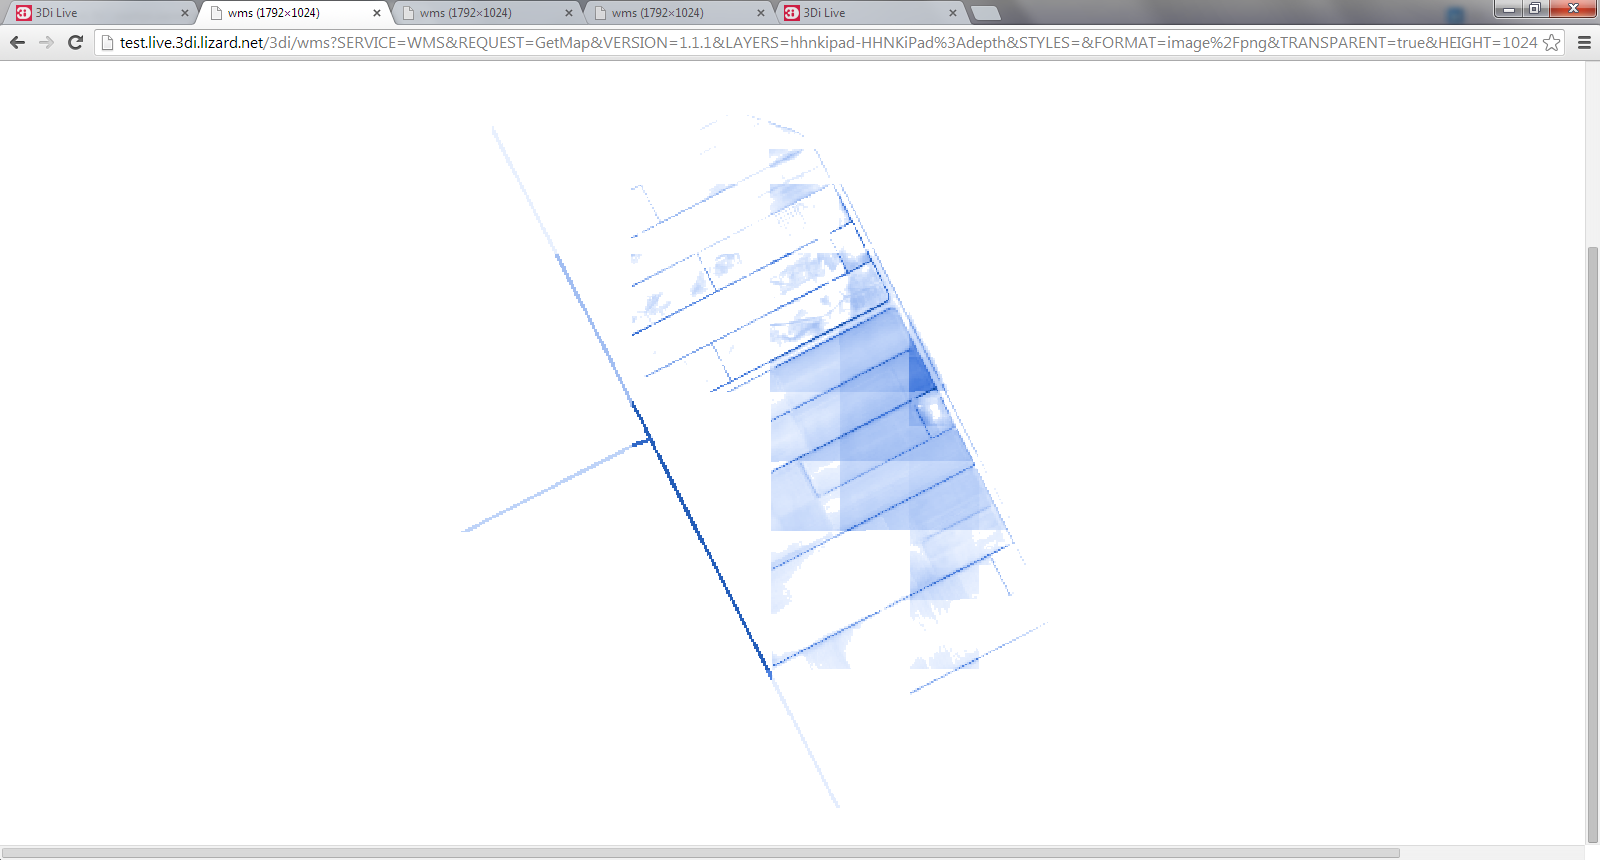
\includegraphics[width=0.5\textwidth]{artifacts_a}
  \caption{Interpolation method}
  \label{fig:artifacts_a}
\end{figure}

\begin{figure}[h]
  \centering
  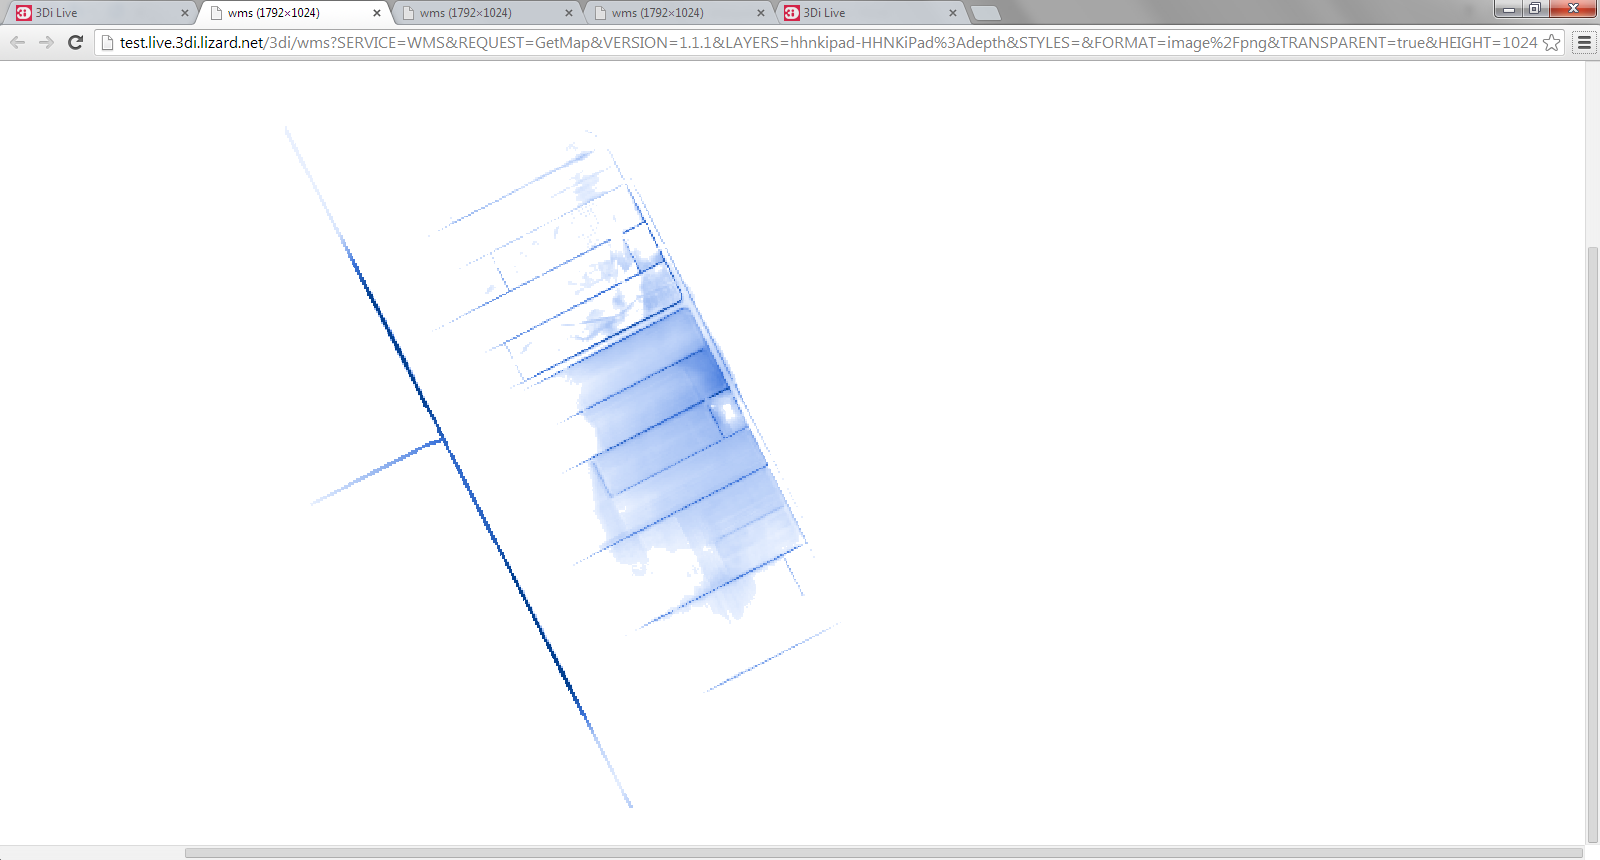
\includegraphics[width=0.5\textwidth]{artifacts_b}
  \caption{Interpolation method}
  \label{fig:artifacts_b}
\end{figure}

Figure 1a.  Artefacts in the visualization                      Figure 1b.  Filtered visualization

A barycentric linear interpolation technique is selected for filtering artefacts on the subgrid level, because of two main restrictions. First, the web visualization requires a 50 ms rendering time in the browser that is still obtained using this method. Second, the ability to interpolate water level results on an arbitrary grid. The quadtree calculation grid was triangulated from the cell centers using existing software libraries, creating a triangulated mesh (Figure 2b). Water level information is present on cell centers and is then linearly interpolated to the underlying subgrid. The interpolation uses a weighted average the determine water levels on the subgrid. The determination of the triangular mesh is very low cost after which the interpolation can be executed immediately. The little calculation steps needed result in high performance. This technique has a large upside in calculation time compared to a technique using cell corners as interpolation points. When using cell corners, an extra intermediate calculation has to be made to determine water levels at cell corners. After the extra calculation the interpolation is executed. Results of plotting water depths after the barycentric linear interpolation are shown in Figure 1b.

The triangulation within the linear barycentric interpolation also allows us to filter levee artefacts of the numerical model .The calculation grid incorporates the function of a levee in the numerical schemes. However it disregards the actual position of such a levee within a calculation cell. The triangulation can reconstruct levees with use of additional levee geometries. A triangle is one of the simplest geometrical forms and can be used reconstruct any arbitrary shape (Welch and Witkin, 1994). To incorporate the levee in the trianglulation, the levee and grid geometries are intersected (Figure 2a). For the intersected calculation cells the influential water level points are determined and coupled to the relevant calculation areas. The arrows in figure 2a indicate which water level is relevant for the dike intersected cell areas. When all waterlevel points are allocated to the dike, the triangulation can be executed with the incorporation of the levee geometries. The newly created triangular mesh now also follows the added levee geometry. Successively the interpolation is executed, resulting in water being retained behind the dike within one calculation cell. The interpolated result is shown in Figure 2b.



\begin{figure}[h]
  \centering
  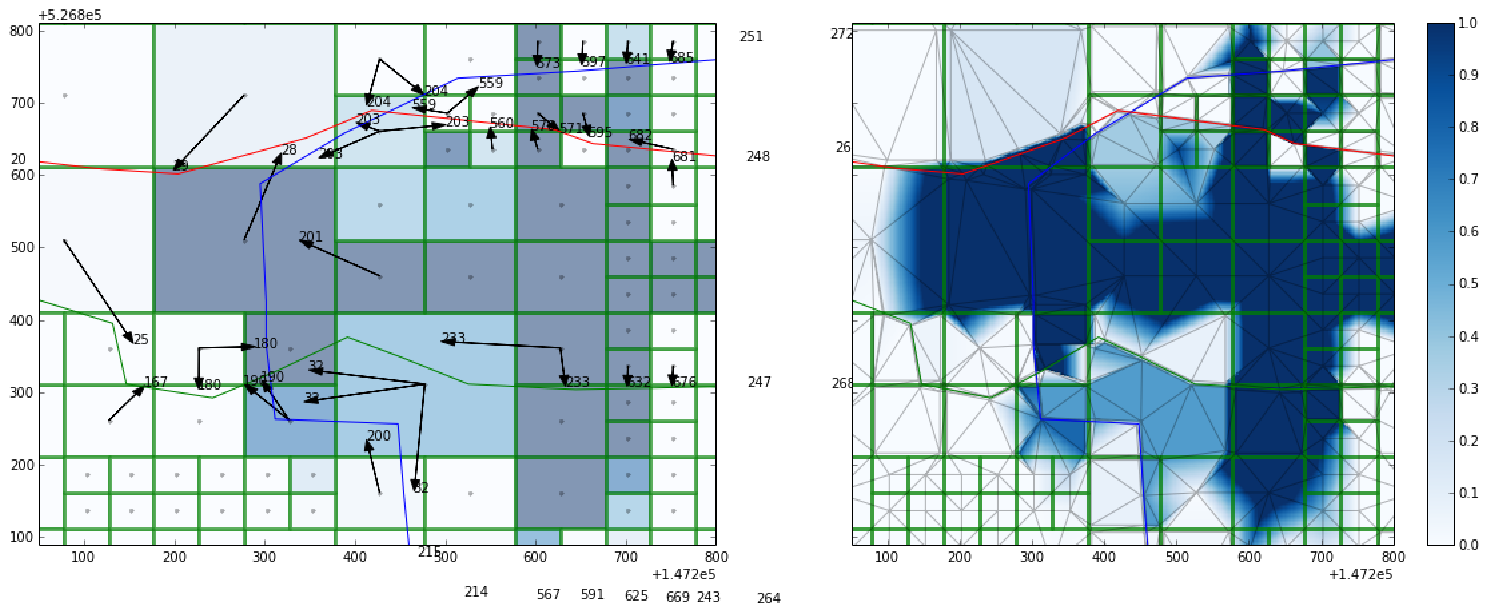
\includegraphics[width=0.5\textwidth]{interpolationlevees3}
  \caption{Interpolation method}
  \label{fig:interp_a}
\end{figure}

Figure 2a. Levee and grid geometry intersections        Figure 2b. Levee incorporated interpolation

Reference:
Welch, W. Witkin, A. Free-Form Shape Design Using Triangulated Surfaces, Proceeding SIGGRAPH '94 Proceedings of the 21st annual conference on Computer graphics and interactive techniques, Pages 247-256, 1994
Stelling, G.S. Quadtree flood simulations with sub-grid digital elevation models, Proceedings of the ICE - Water Management, Volume 165, Issue 10, 01 November 2012, pages 567 –580

http://quietplease.com/home/tri.pdf

\section{Limitations: \emph{All}}
Several other models use similar approaches, albeit with limitations. The subgrid scheme by \citet{Stelling2012} is partly based on the subgrid method for flooding and drying by \citet{Casulli2009}, who implements his methods in the UnTRIM research package \citet{Casulli2000}. UnTRIM uses fully unstructured grids as opposed to the quad tree grids used here. The coupled 1D-2D hydrodynamic model MIKE-FLOOD \citep{Dhi2014} also offers subgrid overland flow. In the accompanying MIKE-SHE all relevant vertical hydrological processes are offered, also with some degree of subgrid-information for the infiltration part.



\section{Future plans: \emph{All}}
In that respect, combining the subgrid approach with our own unstructured flow solver Delft3D-FLOW Flexible Mesh \citep{Kernkamp2011} which is already equipped with an interactive BMI-interface) is a logical future step.
\section{Conclusions: \emph{Fedor}}




%%%%%%%%%%%%%%%%%%%%%%%%%%%%%%%%%%%%%%%%%%%%%%%%%%%%%%%%%%%%%%%%%
\bibliographystyle{iemss}
\bibliography{bibliography}
%%%%%%%%%%%%%%%%%%%%%%%%%%%%%%%%%%%%%%%%%%%%%%%%%%%%%%%%%%%%%%%%%

\begin{acronym}[AAAAA]
\acro{H2O}[$\mathrm{H_2O}$]{water}
\acro{BMI}{Basic Model Interface}
\acro{API}{Application Programming Interface}
\acro{GUI}{Graphical User Interface}
\acro{DEM}{Digital Elevation Model}
\acro{HTTP}{Hyper Text Transfer Protocol}
\acro{IaaS}{Infrastructure as a Service}
\end{acronym}



\end{document}
